\documentclass[en]{../../../../../../eplexam}

\hypertitle{Stochastic processes}{6}{INMA}{1731}{2019}{Septembre}{Majeure}
{Alice Borbáth}
{Pierre-Antoine Absil and Luc Vandendorpe}

\section{}

Find a real-rational transfer function $L(s)$, with all its poles and zeros in the open-left-hand plane, such that, if the input of the causal system with transfer function $L(s)$ is a white noise $E(t)$ with power spectral density $\gamma_E(j\omega) \equiv 1$, then the output $Y(t)$ has power spectral density
$$\gamma_Y(j\omega) = \frac{\omega^4+4}{\omega^4+5\omega^2+4}$$

Justify your answer.

\nosolution

\section{}

Suppose that we would like to estimate a process $d(n)$ from the noisy observations 
$$x(n)=d(n)+v(n)$$.

The power spectral densities $\gamma_d(e^{j\Omega})$ and $\gamma_\nu(e^{j\Omega})$ of $d(n)$ and $v(n)$ are both provided in Figure \ref{fig:pres}

\begin{figure}[h!]
    \centering
    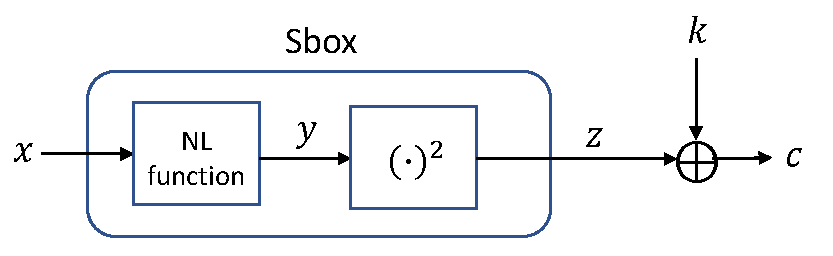
\includegraphics[scale=0.6]{Q2.pdf}
    \caption{Power spectral densities of signal and noise}
    \label{fig:pres}
\end{figure}

We make the following assumptions on the signals :
\begin{itemize}
    \item[-] $d(n)$ and $v(n)$ are both zero mean and wide sense stationary.
    \item[-] the noise v(n) is uncorrelated with $d(n)$.
    \item[-] in Figure \ref{fig:pres}, we assume that $\delta<\frac{\pi}{4}$.
\end{itemize}

We are first interested in designing a first order Wiener filter for estimating $d(n)$ from $x(n)$, that is
$$W(z)=w(0)+w(1)z^{-1}$$

\begin{enumerate}
    \item Obtain the linear system to solve in order to compute the $z$ coefficient as function of $A$, $\delta$ and $N_0$.
\end{enumerate}

We are secondly interested in designing a noncausal Wiener smoothing filter $w(l)$ for estimating $d(n)$ from $x(n)$, that is
$$\hat{d}(n) = \sum_{l=-\infty}^{\infty} w(l)x(n-l)$$

\begin{enumerate}
    \setcounter{enumi}{1}
    \item Compute the expression of the optimum filter.
    \item Compute the resulting MSE. Compare with the MSE that would result from choosing $w(n)=d(n)$.
\end{enumerate}

\nosolution

\end{document}
